\ifdefined\withimages
	\newpage
	\tikz[remember picture,overlay] \node[opacity=1,inner sep=0pt] at (current page.center){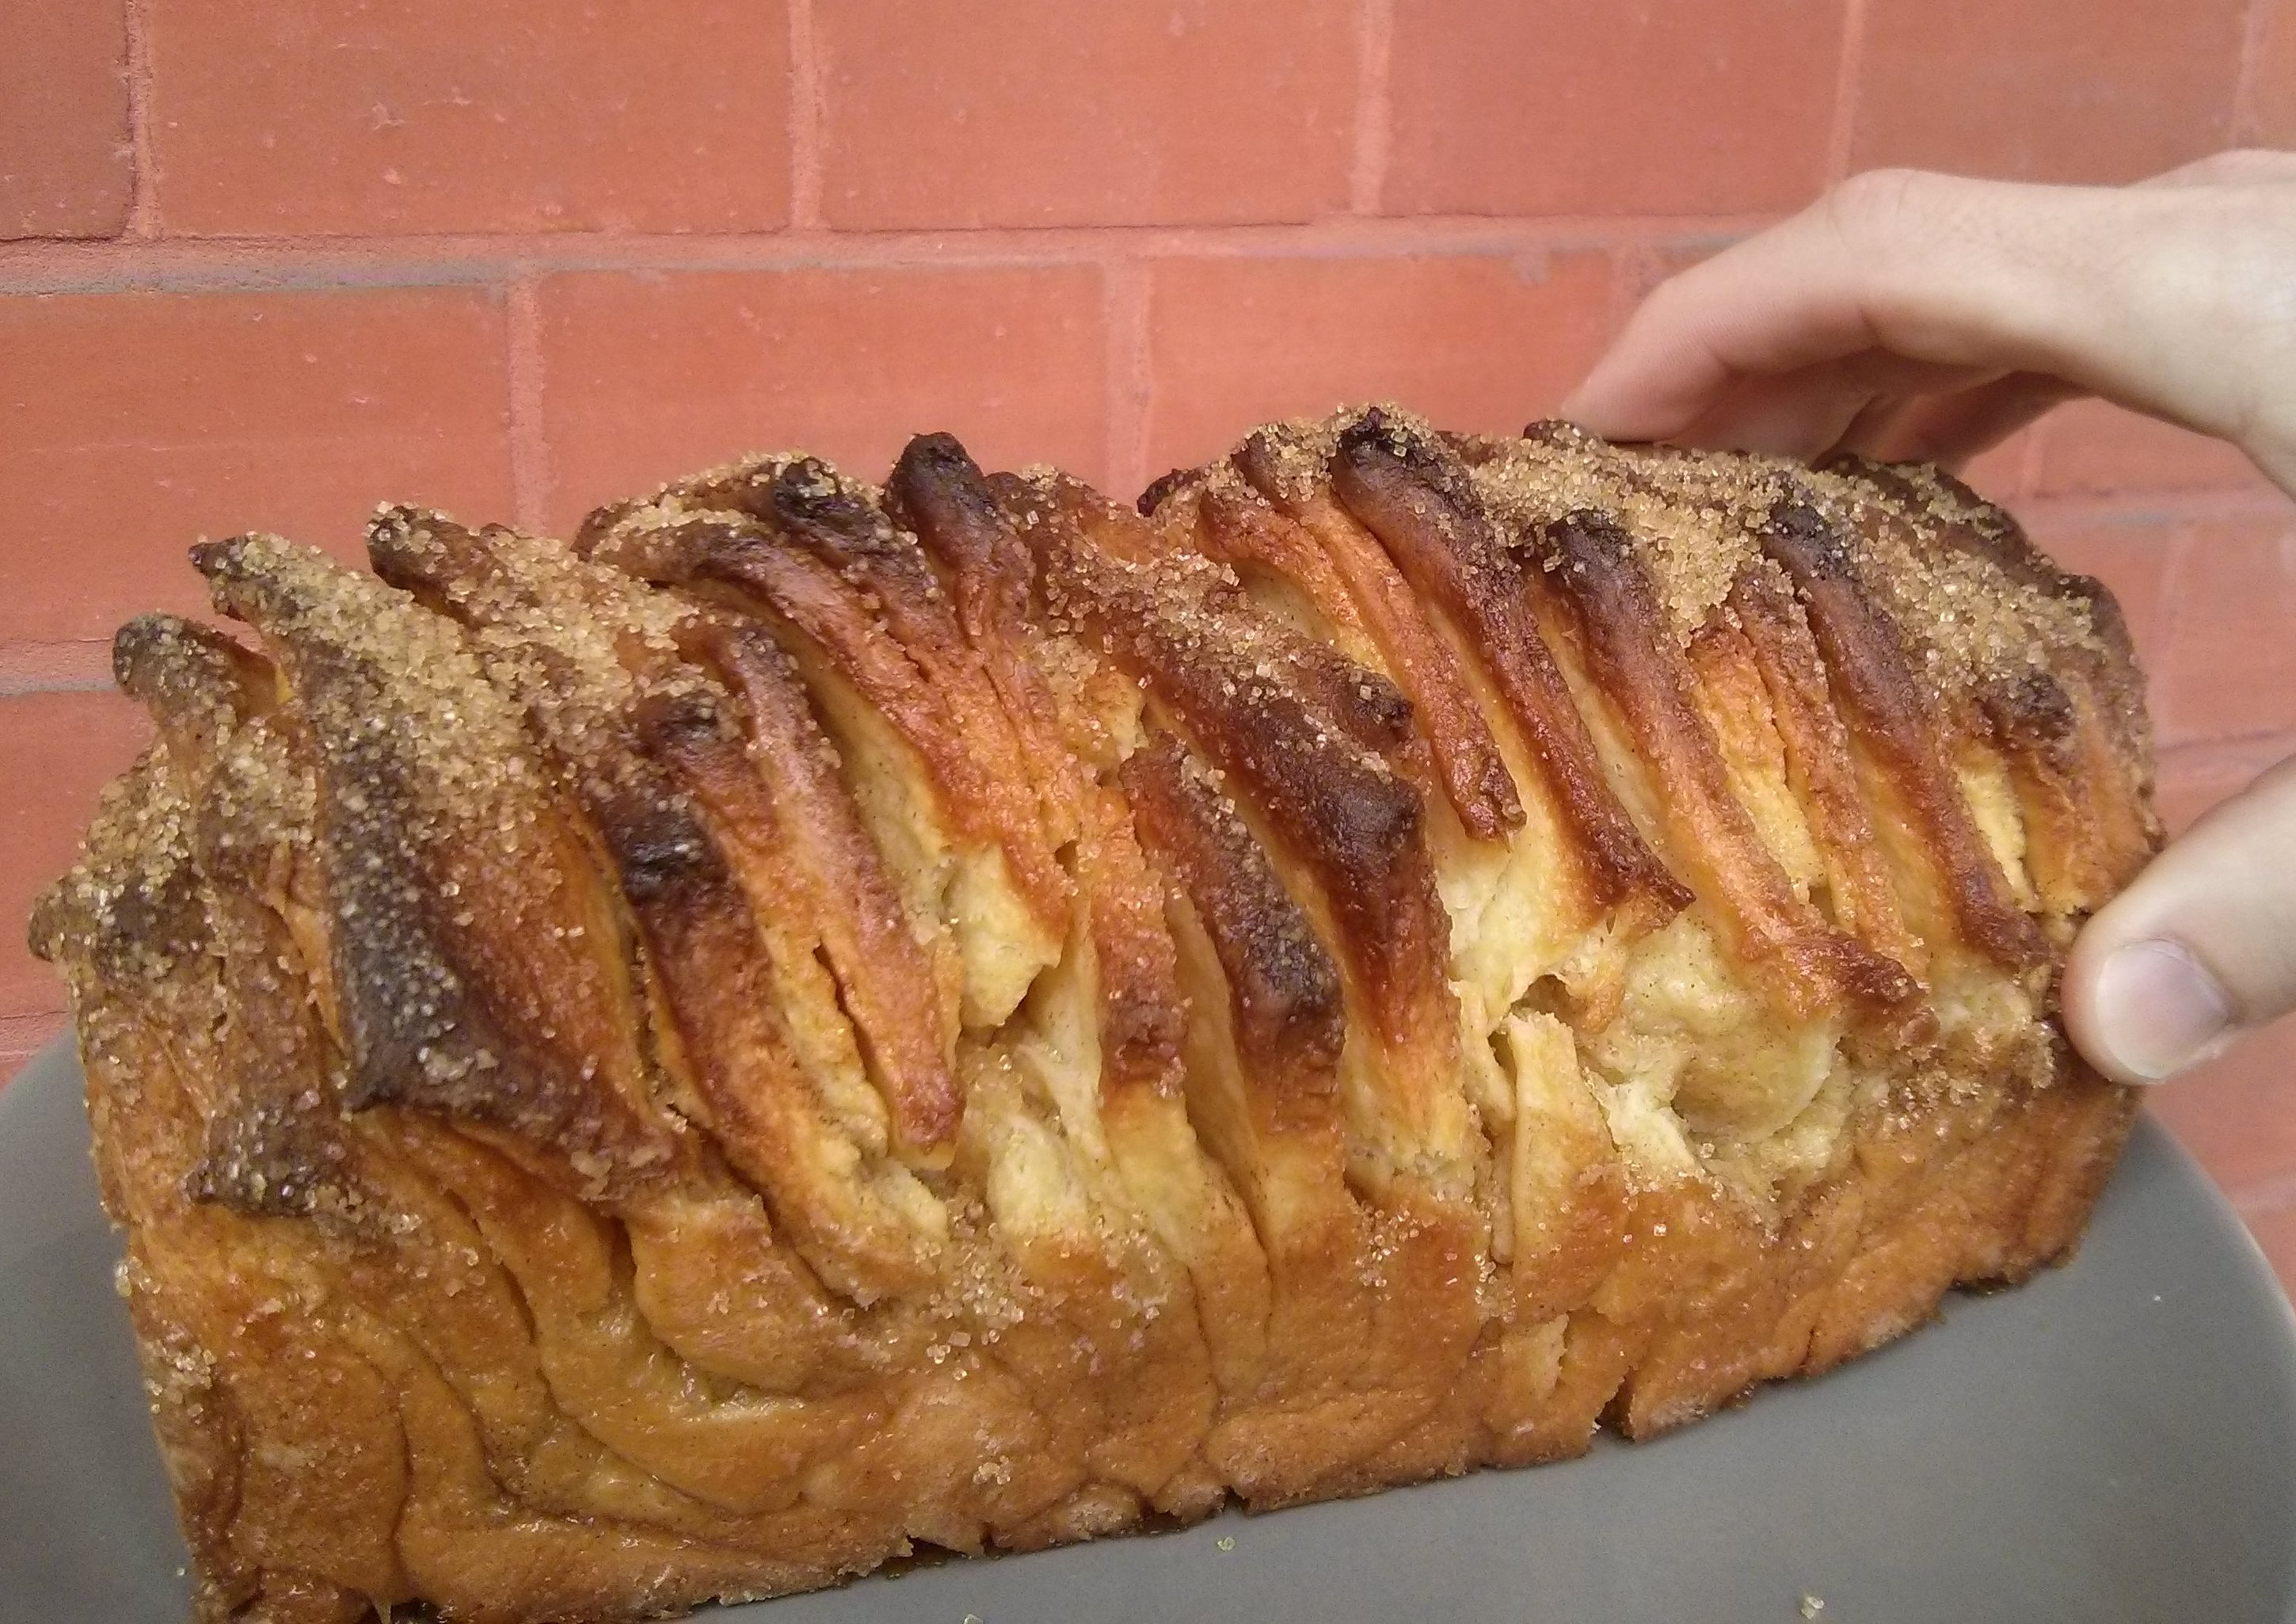
\includegraphics[width=\paperwidth,height=\paperheight]{./bilder/faltenkuchen_ratio.jpg}};
\fi

\begin{recipe}[]{Faltenkuchen} %Quelle
	\timerecipe[Minuten]{ca. 30+180+40} %mit [EINHEIT]
	\personcount[Kastenform (25 cm)]{1} % mit[ART]
	\ingredient{20g frische Hefe} % ggf. \nicefrac{1}{2}
	\ingredient{150ml lauwarme Milch}
	\ingredient{50g Zucker}
	\ingredient{1/2 TL Salz}
	\ingredient{2 Eier}
	\ingredient{375g Mehl}
	\ingredient{125g geschmolzene Butter}
	\ingredient{100g brauner Zucker}
	\ingredient{1 TL Zimt}



\step
\textbf{20g Hefe} in \textbf{150ml lauwarmer Milch} mit einigen Krümeln \textbf{Zucker} auflösen und stehen lassen bis es Blasen bildet.

\step
\textbf{50g Zucker}, \textbf{1/2 TL Salz}, \textbf{2 Eier}, \textbf{375g Mehl} und \textbf{50g geschmolzene Butter} mischen. Die Hefemasse dazu geben, kräftig mit einem Kochlöffel durchschlagen - die Masse ist ziemlich dünn, ist aber richtig so. Den Teig zugedeckt ca. 1 - 1,5 Std. gehen lassen.

\step
Den Teig auf einer bemehleten Fläche ca. 1/2 cm - 1cm dick ausrollen, danach mit einem Pinsel mit \textbf{75g geschmolzener Butter} bestreichen (1 EL von der Butter für später aufheben). \textbf{100g braunen Zucker} mit \textbf{1 TL Zimt} mischen auf dem ausgerollen Teig verteilen (1 EL von der Zimt-Zuckermischung  für später aufheben).

\step
Den Teig in der breite der Kuchenform in Streifen schneiden. Diese Streifen jetzt in der Höhe der Kuchenform in Vierecke schneiden, diese Vierecke übereinander schichten zu Paketen und in der Kastenform hintereinander setzten. Den Teig in der Form nochmals 30 Minuten gehen lassen.

\step
Im vorgeheizten Ofen bei 180 Grad auf der zweiten Schiene von unten 30-40 Minuten backen. Den noch warmen Kuchen mit einem Pinsel mit der restlichen flüssigen Butter bestreichen und mit der restlichen Zimt-Zuckermischung bestreuen. 

%\tippbox{\textbf{Tipp:} ...} % Tipp in extra Rahmen
\end{recipe}